\section{Exercises}
\subsection{Quantitative Process Analysis}
Usually, in this type of exercises, you are given a process model, enriched with branching probabilities, along with
a table containing the cycle time and processing time measures for each activity.
\\Take the following process as an example:
\begin{figure}[H]
    \centering
    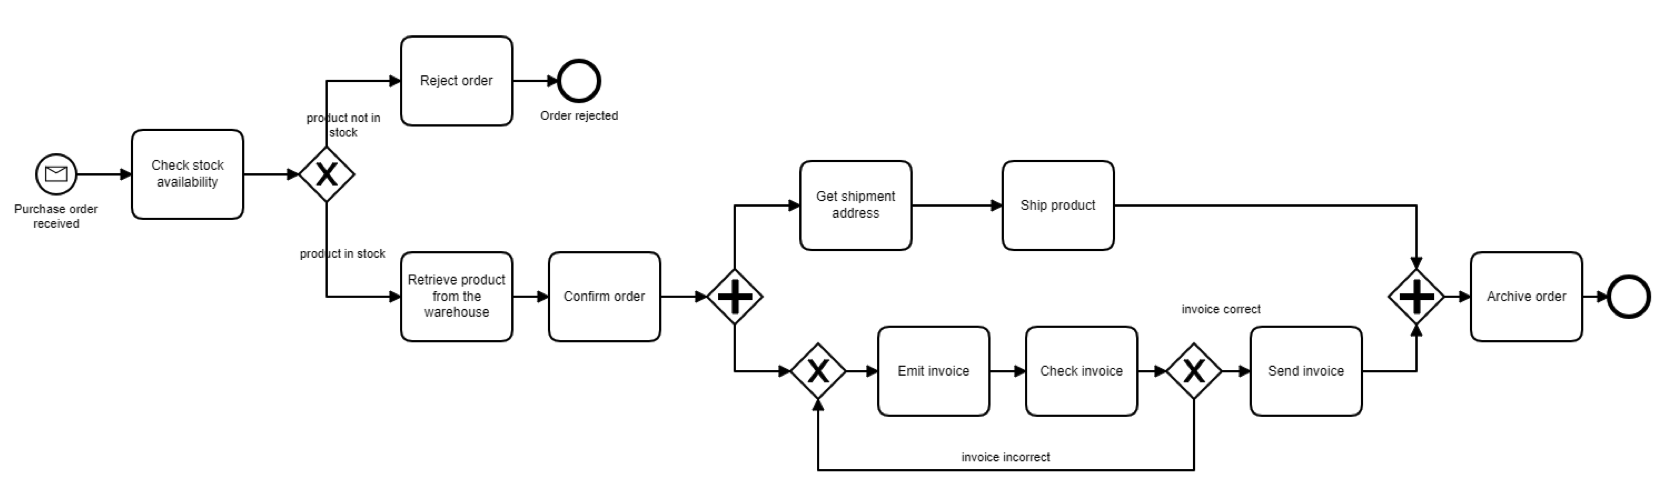
\includegraphics[width=\textwidth]{images/exercises/q_a_bpnm.png}
    \caption{Example Process for Quantitative Analysis Exercises}
\end{figure}
\begin{itemize}
    \item 20\% of the orders are rejected for product not in stock;
    \item 10\% of the orders have an incorrect invoice;
\end{itemize}
and the following table:
\begin{table}[H]
    \centering
    \resizebox{0.8\textwidth}{!}{%
        \begin{tabular}{c|c|c}
            \hline
            \textbf{Activity} & \textbf{Cycle Time (CT)} & \textbf{Processing Time (PT)} \\
            \hline
            Check stock availability & 1 day & 30 min \\
            Reject order & 7 days & 1 hour \\
            Retrieve product from the warehouse & 3 days & 4 hours \\
            Confirm order & 4 days & 2 hours \\
            Get shipment address & 1 day & 30 min \\
            Ship product & 10 days & 24 hours \\
            Emit invoice & 1 day & 1 hour \\
            Check invoice & 1 day & 30 min \\
            Send invoice & 2 days & 30 min \\
            Archive order & 4 days & 1 hour \\
            \hline
        \end{tabular}
    }
\end{table}
Using the information provided, compute the following:
\begin{enumerate}
    \item The \textbf{Cycle Throughput Time} of the process;
    \item The \textbf{Cycle Time} of the process;
    \item The \textbf{Cycle Time Efficiency (CTE)} of the process;
\end{enumerate}
\paragraph{Solution:}
\begin{enumerate}
    \item The Cycle Throughput Time can be computed with the rules provided in the \ref{fig:cycle_time_table}. The resulting equation is:
    \[CT = 1 + (7 \times 0.2) + \left[\left(3 + 4 + \max\left(1 + 10, \frac{(1 + 1)}{0.9} + 2\right) + 4 \right) \times0.8\right]\]
    \[ = 1+ 1.4 + \left[(3 + 4 + 11 + 4) \times 0.8\right] = 2.4 + 17.6 = 20 \text{ days}\]
    \item The Processing Time can be computed similarly, simply substituting the cycle times with processing times:
    \[PT = 0.5 + (1 \times 0.2) + \left[\left(4 + 2 + \max\left(0.5 + 24, \frac{(1 + 0.5)}{0.9} + 0.5\right) + 1 \right) \times0.8\right]\]
    \[ = 0.5 + 0.2 + \left[(4 + 2 + 24.5 + 1) \times 0.8\right] = 0.7 + 6 \times 0.8 = 0.7 + 25.2 = 25.9 \text{ hours}\]
    \item Finally, we can compute the Cycle Time Efficiency as:
    \[CTE = \frac{PT}{CT} = \frac{25.9 \text{ hours}}{20 \text{ days}} = \frac{25.9}{20 \times 8} = 16\%\]
\end{enumerate}
